\documentclass{beamer}
\usetheme{metropolis}
\usepackage{ctex}
\usepackage{caption}
\usepackage{subfigure}

\title{Item-Based Collaborative Filtering}
\date{\today}
\author{Yang LI}
\institute{School of Software Engineering, Tongji University}

\begin{document}
  \maketitle
  \section{Chinese Text Segmentation}
  \begin{frame}{中文分词框架选择}
  \begin{itemize}
    \item Jieba
    \item THULAC
    \item IK Analyzer
    \item Stanford
  \end{itemize}
  \end{frame}
  \begin{frame}{分词算法的分类}
    \begin{columns}
      \begin{column}{0.5\textwidth}
          基于词典
          \begin{itemize}
            \item 正向最大匹配
            \item 逆向最大匹配
            \item 双向匹配
          \end{itemize}
      \end{column}
      \begin{column}{0.5\textwidth}
        基于统计
        \begin{itemize}
          \item HMM
          \item CRF
          \item SVM
          \item DL
        \end{itemize}
      \end{column}
    \end{columns}
  \end{frame}
  \begin{frame}{分词结果}
    \begin{figure}
      \centering
      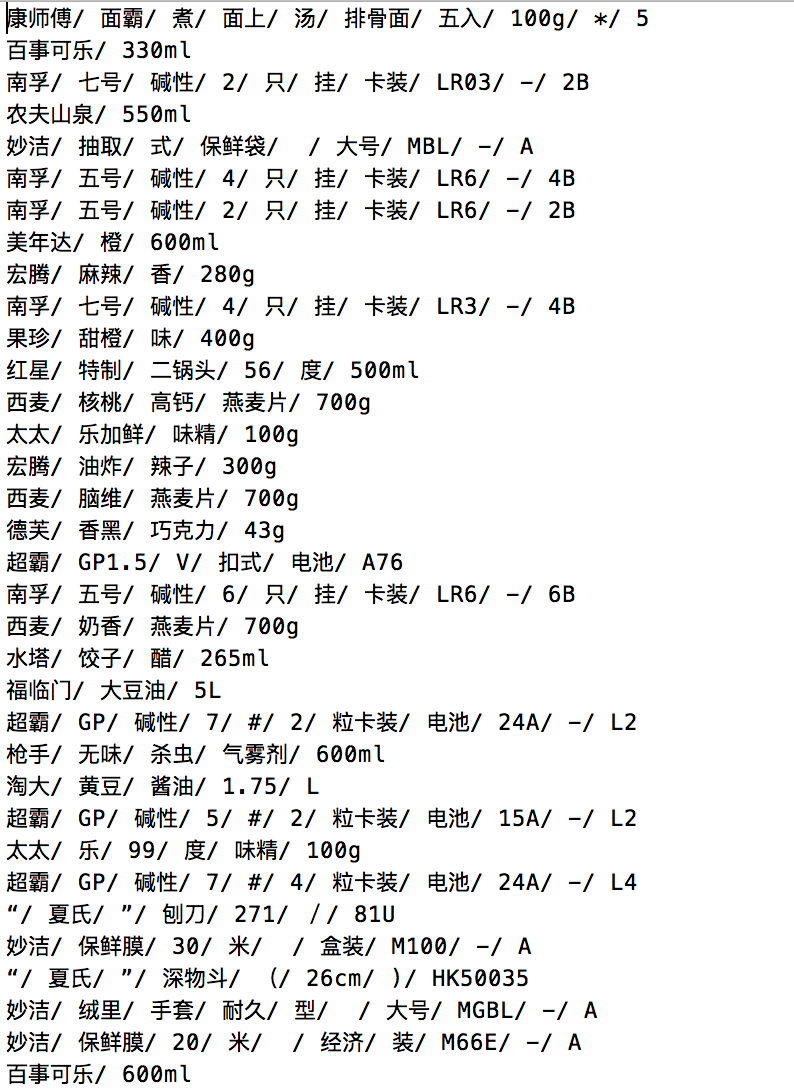
\includegraphics[width=\textwidth]{Nov-9/result}
    \end{figure}
  \end{frame}
  \begin{frame}{一些具体的改进} 
    \begin{itemize}
      \item 根据词性删除了没有太多意义的副词、数量词等
      \item 后题考虑增加关键词的筛选(TextRank Algorithms, 基于PageRank)
      \item 与多个信息(商品品牌、商品单位、包装类型)结合处理
    \end{itemize}
  \end{frame} 
  \section{Similarity}
  \begin{frame}{计算相似度}
    \begin{columns}
      \begin{column}{0.5\textwidth}
        原始
        \begin{itemize}
          \item 对每一个用户每次购买的东西增加一个相似度
          \item 最后除以总量(归一化)
        \end{itemize}
      \end{column}
      \begin{column}{0.5\textwidth}
        现在
        \begin{itemize}
          \item 对于同一大类的商品
          \item 对商品名进行分词
          \item 分词结果计算Levenshtein Distance(Smith-Waterman algorithm,  Needleman–Wunsch algorithm)
          \item 对距离进行处理(取倒数, 归一化, 高斯函数)
        \end{itemize}
      \end{column}
    \end{columns}
  \end{frame}
  \begin{frame}{结果}
    precision
    \begin{figure}
      \centering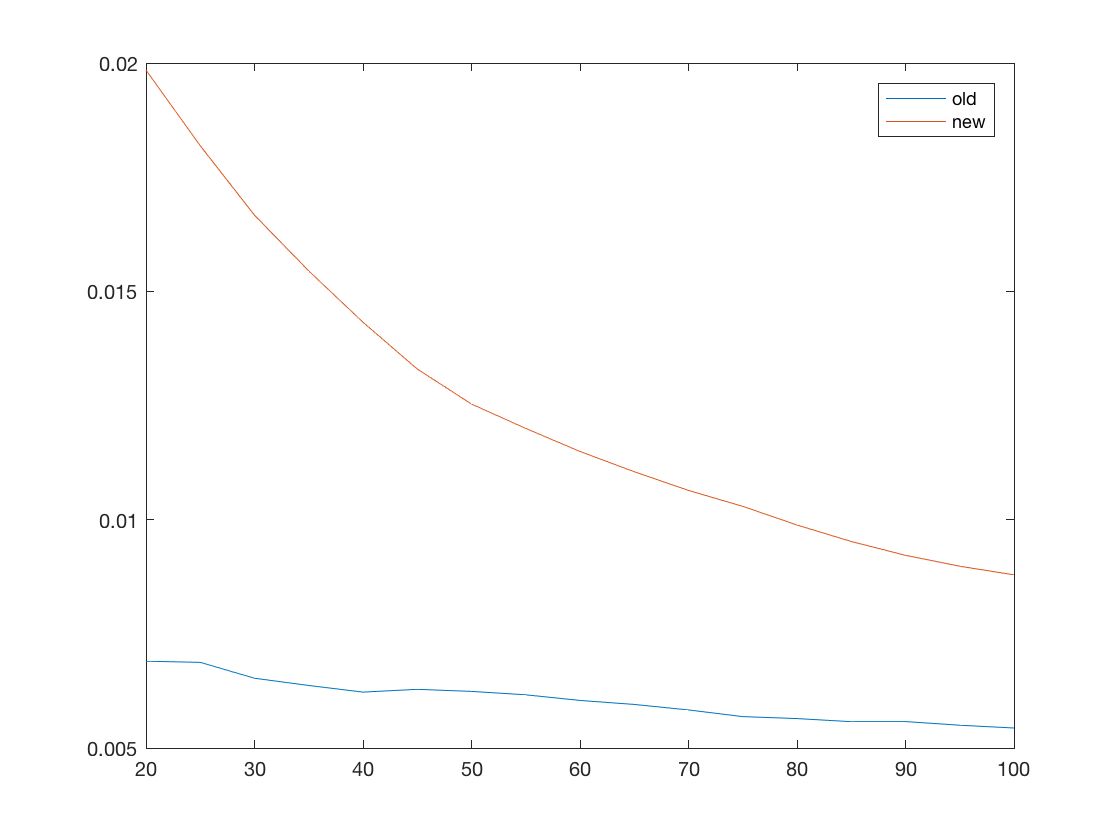
\includegraphics[width=0.9\textwidth]{Nov-9/result_1.png}
    \end{figure}
  \end{frame}
  \begin{frame}{结果}
    recall
    \begin{figure}
      \centering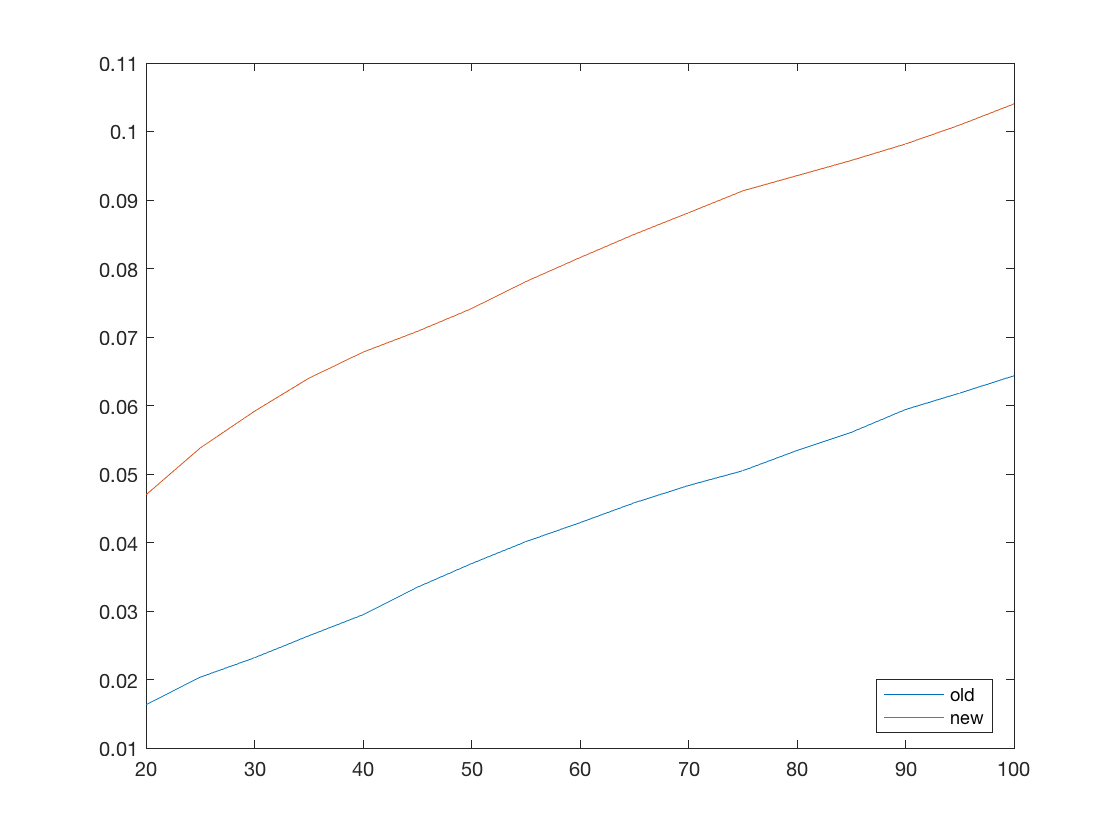
\includegraphics[width=0.9\textwidth]{Nov-9/result_2.png}
    \end{figure}
  \end{frame}
  \begin{frame}{问题}
    \begin{itemize}
      \item 评价指标(precision, recall?)
      \item 分词结果的准确性
      \item 对距离的处理
    \end{itemize}
  \end{frame}
\end{document}
